\documentclass{beamer}
\mode<presentation>
\usetheme{CambridgeUS}
\usepackage[russian]{babel}
\usepackage[utf8]{inputenc}
\usepackage[T2A]{fontenc}
\usepackage{sansmathaccent}

\usepackage{verbatim}
\usepackage{alltt}

\pdfmapfile{+sansmathaccent.map}
\title[Основы языка Pascal]{Разветвляющиеся вычислительные процессы}
\author{Наумов Д.А., доц. каф. КТ}
\date[03.10.2019] {Программирование и алгоритмические языки, 2019}

\begin{document}

%ТИТУЛЬНЫЙ СЛАЙД
\begin{frame}
  \titlepage
\end{frame}
  
%СОДЕРЖАНИЕ ЛЕКЦИИ
\begin{frame}
  \frametitle{Содержание лекции}
  \tableofcontents  
\end{frame}

\section{Разветвляющиеся алгоритмы}

\begin{frame}{Разветвтляющиеся алгоритмы}
\begin{block}{Разветвляющийся вычислительный процесс}
в зависимости от выполнения определенных условий реализуется по одному из нескольких заранее предусмотренных направлений. 
\end{block}
\begin{itemize}
\item Каждое отдельное направление называется - \textbf{ветвью вычислений}. 
\item Выбор той или иной ветви осуществляется уже \textbf{при выполнении программы }в результате проверки \textbf{некоторых условий }и определяется свойствами исходных данных и промежуточных результатов. 
\end{itemize}
\begin{figure}[h]
\centering
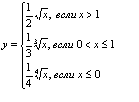
\includegraphics[scale=1]{images/lec03-pic01.png}
\end{figure}
\end{frame} 

\begin{frame}[fragile]{Тип Boolean}
Для реализации разветвляющих алгоритмов в языке Pascal предусмотрен специальный тип данных - \emph{логический}. 
Переменная логического типа описывается следующим образом: 
\begin{alltt}
1 var
2   ИмяПеременной: Boolean; 
\end{alltt}
Переменная логического типа может принимать одно из двух значений: 
\begin{itemize}
\item логическая ложь (константа логического типа False);
\item логическая истина (константа логического типа True);
\end{itemize}
Значение типа Boolean можно вывести операторами write/writeln, но нельзя считать операторами read/readln.
\end{frame}

\begin{frame}[fragile]{Операции отношения}
Для задания условия в логическом выражении используются операции отношения. 
\begin{block}{Операции отношения}
Операция отношения – это конструкция вида $A\Theta B$, где 
\begin{itemize}
\item A и B – любые выражения языка ActionScript, 
\item $\Theta$ – знак операции отношения.
\end{itemize}
Допустимы следующие операции отношения:
\begin{itemize}
\item $<$ (меньше), 
\item $<=$ (меньше или равно), 
\item $>$ (больше), 
\item $>=$ (больше или равно), 
\item $=$ (равно), 
\item $<>$ (не равно)
\end{itemize}
\end{block}
\end{frame}

\begin{frame}[fragile]{Пример}
\begin{itemize}
\item результат вычисления выражения 4 > 5 равен false;
\item результат вычисления выражения 2 >= 2 равен true;
\item результат вычисления выражения 9 !=0  равен true;
\end{itemize}
\begin{alltt}
1 var x, y: real;
2 begin
3  x := 0.1;
4  x := x + 0.1; x := x + 0.1;
4  x := x + 0.1; x := x + 0.1;
5  y := 1/2;
6  writeln(x=y); //результат false!
7  readln;
8 end.
\end{alltt}
\end{frame}

\begin{frame}[fragile]{Пример. Сравнение двух вещественных чисел}
\begin{itemize}
\item вводится величиная погрешности, которая будет использоваться при сравнении чисел;
\item два числа будут считаться равными (приблизительно), если модуль их разности не превышает погрешность.
\end{itemize}
\[|X - Y| < \varepsilon\]
\begin{alltt}
1 const eps = 1e-6;
1 var x, y: real;
2 begin
3   x := 0.1;
4   x := x + 0.1; x := x + 0.1;
4   x := x + 0.1; x := x + 0.1;
5   y := 1/2;
6   writeln(abs(x-y)<eps); //результат true
7   readln;
8 end.
\end{alltt}
\end{frame}

\begin{frame}[fragile]{Логические операции}
Для объединения нескольких логических выражений использу-ют логические операции: 
\begin{itemize}
\item not A - отрицание;
\item A and B - конъюнкция (логическое умножение); 
\item A or B - дизъюнкция (логическое сложение);
\item A xor B - сложение по модулю 2 (исключающее или);
\end{itemize}
A и B - выражения логического типа, тип результата - логический.
\begin{figure}[h]
\centering
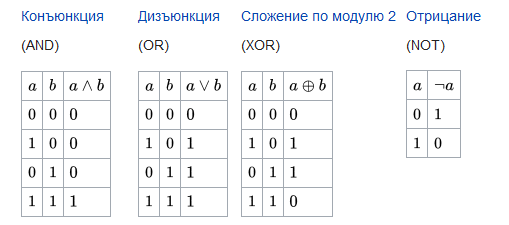
\includegraphics[scale=0.5]{images/lec03-pic02.png}
\end{figure}
\end{frame}

\begin{frame}[fragile]{Пример. Сравнение двух вещественных чисел}
\begin{itemize}
\item вводится величиная погрешности, которая будет использоваться при сравнении чисел;
\item два числа будут считаться равными (приблизительно), если модуль их разности не превышает погрешность.
\end{itemize}
\[|X - Y| < \varepsilon\]
\begin{alltt}
1 const eps = 1e-6;
1 var x, y: real;
2 begin
3   x := 0.1;
4   x := x + 0.1; x := x + 0.1;
4   x := x + 0.1; x := x + 0.1;
5   y := 1/2;
6   writeln(abs(x-y)<eps); //результат true
7   readln;
8 end.
\end{alltt}
\end{frame}

\begin{frame}[fragile]{Приоритет операций}
\begin{itemize}
\item действия в скобках; 
\item $not;$
\item $*, /, div, mod, and, shr, shl;$
\item $+, -, or, xor;$
\item $=, <>, >, <, >=, <=$;
\end{itemize}
\begin{alltt}
1 var x, y: integer;
2 begin
3   x = 8; y = -1; 
4   writeln(0 < x < 10);            // ошибка
5   writeln(0 < x and x < 10);      // ошибка
6   writeln((0 < x) and (x < 10));  // ошибка 
7   writeln((0 < x) and (x < 10));  // нет ошибки
8   writeln(x and y);               // ?
9 end.
\end{alltt}
\end{frame}

\begin{frame}
\textbf{Разветвляющийся вычислительный процесс}, содержащий две ветви, схематично может быть изображен с помощью структуры выбора (структуры разветвления), которая содержит три элемента: 
\begin{itemize}
\item логическое условие, 
\item ветвь <<ДА>>, 
\item ветвь <<НЕТ>>.
\end{itemize}
\begin{figure}[h]
\centering
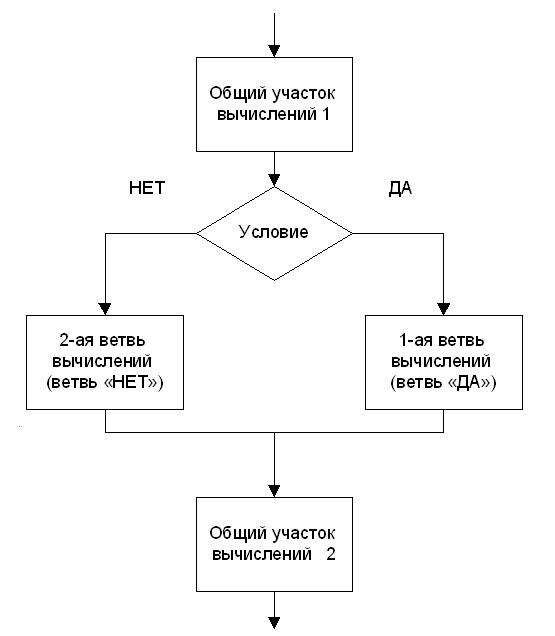
\includegraphics[scale=0.35]{images/lec03-pic03.png}
\end{figure}
\end{frame}

\begin{frame}[fragile]{Условный оператор}
\begin{alltt}
1 if выражение then
2    оператор1
3 else
4    оператор2;
\end{alltt}
\begin{itemize}
\item выражение - выражение \textit{логического типа};
\item оператор1, оператор2 - (одиночные) операторы языка Паскаль.
\end{itemize}
Порядок выполнения условного оператора:
\begin{enumerate}
\item вычисляется значение \textit{логического выражения};
\item если значение логического выражения равно \textbf{true}, то выполняется Оператор1 (а Оператор2 пропускается);
\item если значение логического выражения равно \textbf{false}, то выполняется Оператор2 (а Оператор1 пропускается);
\item выполняется оператор, стоящий в программе непосредственно после оператора \textit{if}.
\end{enumerate}
\end{frame}

\begin{frame}[fragile]{Пример}
Вычисление функции по одной из двух предложенных формул в зави-симости от значения аргумента
\begin{figure}[h]
\centering
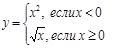
\includegraphics[scale=1]{images/lec03-pic04.png}
\end{figure}
Оператор, реализующий эти вычисления для некоторого значения аргумента х, выглядит следующим образом:
\begin{alltt}
1 if x < 0 then
2    y := x * x
3 else
4    y := sqrt(x);
\end{alltt}
\end{frame}

\begin{frame}[fragile]{Пример}
Задача для определения, можно ли построить треугольник из отрезков заданной длины: x, y, z (x > 0, y  > 0, z > 0).
\begin{figure}[h]
\centering
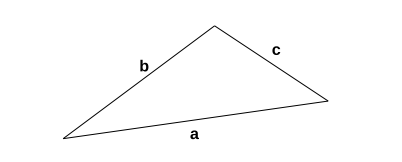
\includegraphics[scale=0.5]{images/lec03-pic05.png}
\end{figure}
Оператор, реализующий эти вычисления для некоторого значения аргумента х, выглядит следующим образом:
\begin{alltt}
1  if (x +y > z) and (x +z > y) and (y +z > x)
2    writeln('треугольник построить можно')
3  else
4    writeln('треугольник построить нельзя');
\end{alltt}
\end{frame}

\begin{frame}[fragile]{Сокращенная форма условного оператора}
\begin{alltt}
1 if выражение then
2    оператор1;
\end{alltt}
\begin{itemize}
\item выражение - выражение \textit{логического типа};
\item оператор1 - (одиночный) оператор языка Паскаль.
\end{itemize}
Порядок выполнения условного оператора:
\begin{enumerate}
\item вычисляется значение \textit{логического выражения};
\item если значение логического выражения равно \textbf{true}, то выполняется Оператор1;
\item выполняется оператор, стоящий в программе непосредственно после оператора \textit{if}.
\end{enumerate}
\end{frame}

\begin{frame}[fragile]{Пример}
Даны три неравных числа a, b, c. Вычислить и напечатать значение z, равное квадрату большего из них.
\begin{figure}[h]
\centering
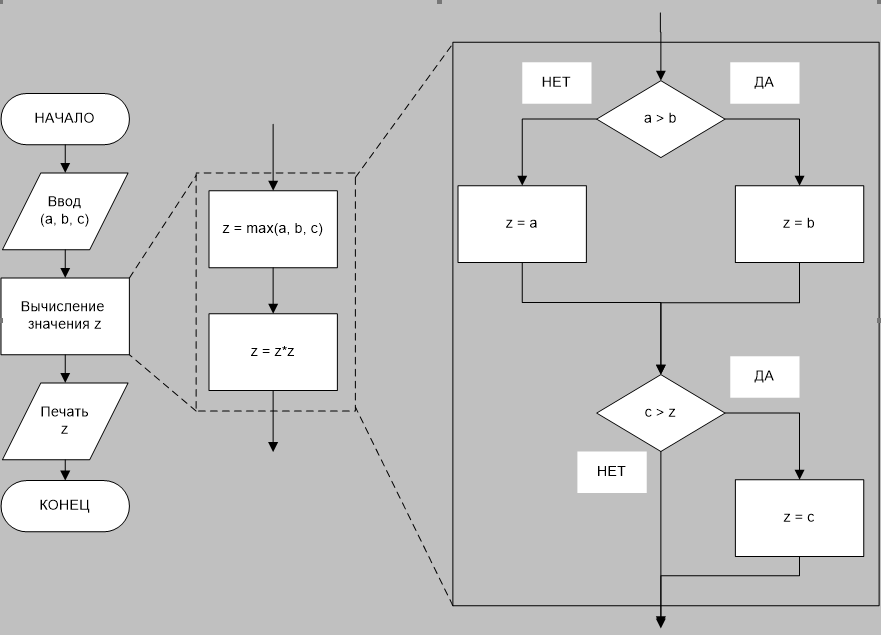
\includegraphics[scale=0.35]{images/lec03-pic06.png}
\end{figure}
\end{frame}

\begin{frame}[fragile]{Вложенные операторы if}
Условные операторы могут иметь вложенную конструкцию, когда в качестве Оператора1 или Оператора2 может также использоваться условный оператор. 
\begin{block}{Правило для вложенных операторов}
ключевое слово \textbf{else} всегда относится к ближайшему предыдущему оператору \textbf{if}.
\end{block}
\begin{alltt}
1 z := 0;
2 if x < 0 then
3    if y < 0 then
4       z := 1
5 else
6    z := 2; // в каких случаях z будет равно 2?
\end{alltt}
\end{frame}

\begin{frame}[fragile]{Пример}
Вычислить значение функции по одной из предложенных формул.
\begin{figure}[h]
\centering
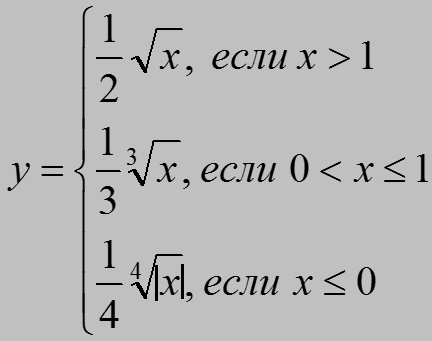
\includegraphics[scale=0.35]{images/lec03-pic07.png}
\end{figure}
\begin{alltt}
1 if x > 1 then
2    y := 1/2 * sqrt(x)
3 else
4   if x > 0 then
5     y := 1/3 * exp(1/3*ln(x))
6   else
7     y := 1/4 * exp(1/4*ln(abs(x)));
\end{alltt}
\end{frame}

\begin{frame}[fragile]{Составной оператор}
В состав условного оператора может входить только один оператор. Если в какую-либо ветвь разветвления требуется вставить несколько операторов, то они объединяются в один, составной оператор:
\begin{alltt}
1 begin
2   оператор1;
3   оператор2;
4   ...
5   операторN;
6 end
\end{alltt}
Элементами составного оператора могут быть любые операторы языка, в том числе и другие составные операторы.
\end{frame}

\begin{frame}[fragile]{Пример}
Вычислить корни квадратного уравнения общего вида.
\begin{figure}[h]
\centering
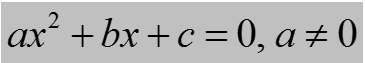
\includegraphics[scale=0.35]{images/lec03-pic08.png}
\end{figure}
Введем обозначения:
\begin{figure}[h]
\centering
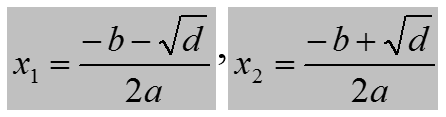
\includegraphics[scale=0.35]{images/lec03-pic09.png}
\end{figure}
\begin{itemize}
\item A, B, C - коэффициенты уравнения;
\item D - дискриминант;
\item X1, X2  -корни уравнения.
\end{itemize}
\end{frame}

\begin{frame}[fragile]{Блок-схема}
\begin{figure}[h]
\centering
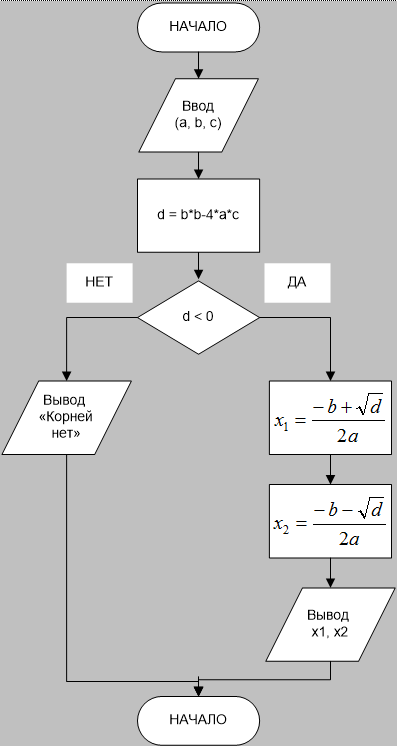
\includegraphics[scale=0.35]{images/lec03-pic10.png}
\end{figure}
\end{frame}

\begin{frame}[fragile]{Фрагмент программы}
\begin{figure}[h]
\centering
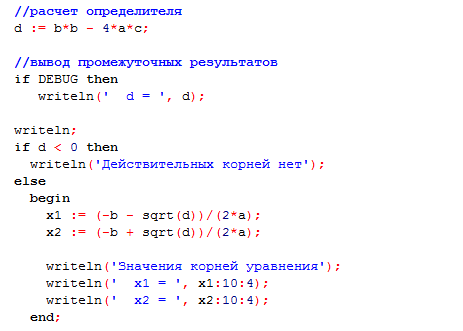
\includegraphics[scale=0.75]{images/lec03-pic11.png}
\end{figure}
\end{frame}

\end{document}
